% Full draft. Numbers come from results/ via report/analysis.py (see notebook/CE893_evaluation.ipynb).
\begin{center}
\vspace*{1.6cm}
{\small CE893-7-AU-CO \textbar{} Generative Artificial Intelligence}\par
\vspace{1.1cm}
{\Huge\bfseries\color{essexpurple}Moving the Harness into the Weights:\\[0.2em] LoRA versus Prompt Engineering for a Text-to-Cube Agent}\par
\vspace{0.5cm}
{\Large Fine-tuning (compared with a prompt-engineering harness)}\par
\vspace{1.4cm}
\begin{tabular}{rl}
\textbf{Student name:} & Shamir Dimaano, [registration number]\\
\textbf{Code and data:} & \url{https://github.com/shamx9ir/msc-ce893}
\end{tabular}
\vfill
\begin{minipage}{0.88\linewidth}
\color{essexpurple}\rule{\linewidth}{1.2pt}\par\smallskip
\textbf{Summary.} A local Qwen2.5-Coder model answers questions about a database by writing queries for a Cube semantic layer, inside a tool-using agent built with Google's ADK. Fine-tuning the same model with a LoRA adapter, while keeping the prompt and tools identical, raised strict execution accuracy on 332 held-out BIRD questions from 27.7\% to 46.4\% (7B) and from 28.9\% to 49.7\% (14B). A LoRA trained on a shorter prompt kept most of that gain while sending 2.4 times fewer prompt tokens per model call.
\par\smallskip\color{essexpurple}\rule{\linewidth}{1.2pt}
\end{minipage}
\end{center}
\clearpage

\section{Introduction and related work}

\subsection{Motivation and context}
Business users ask questions such as \emph{``How many races were held in Italy?''} and expect a number or a chart, not SQL. Many analytics stacks put a \textbf{semantic layer} between the data and its users: Cube~\cite{cube} defines \emph{cubes} (tables), \emph{dimensions} (columns to group or filter by) and \emph{measures} (aggregates such as \texttt{count} or \texttt{avg\_price}) and answers JSON queries by writing the SQL itself, joins included. An LLM that writes Cube queries instead of SQL works on a smaller, safer language, and the result can go straight to a chart.

The model must use member names that exist, put each field in the right slot (a year is a dimension, not a measure), copy stored values exactly and call tools in order. A prompt can explain all of this, but every rule and schema line is paid for again on every model call.

\subsection{Related work}
Text-to-SQL benchmarks moved from Spider~\cite{yu2018spider} to BIRD~\cite{li2023bird}, which adds large real databases, dirty values and an ``evidence'' hint per question, and scores \emph{execution accuracy}. Prompt-only systems such as DIN-SQL~\cite{pourreza2023din} decompose the task and self-correct, and agent loops in the style of ReAct~\cite{yao2023react} let the model test a query before answering; our harness follows this route. Fine-tuned open models such as CodeS~\cite{li2024codes} reach strong BIRD scores at small sizes, and Gorilla~\cite{patil2023gorilla} showed that fine-tuning teaches correct API calls better than prompting alone. LoRA~\cite{hu2021lora} and QLoRA~\cite{dettmers2023qlora} make this possible on one consumer GPU. Finally, \emph{context distillation}~\cite{askell2021general,snell2022distilling} trains a model to behave as if a long prompt were present, which is the idea we test for the harness prompt.

\subsection{Research question and contribution}
\resultplaceholder{\textbf{RQ.} When the same agent harness (prompt + tools) is kept fixed, how much does a LoRA adapter trained on verified tool-use transcripts improve execution accuracy on unseen databases, and how much of the prompt (query guide, tool definitions, schema) can the adapter replace without losing accuracy? A second question: how much does each setup depend on BIRD's hint?}

We built (i) a Cube semantic layer and an ADK agent for BIRD databases, (ii) a pipeline that turns BIRD training SQL into 3,531 execution-verified Cube transcripts, (iii) LoRA adapters for Qwen2.5-Coder 7B and 14B~\cite{hui2024qwen25coder} under three prompt profiles, and (iv) a demo app that shows answers as Highcharts charts through A2UI~\cite{a2ui}. Every arm runs the same 4-bit model file in Ollama, so arms differ only in the adapter and the prompt.

\begin{figure}[!htbp]
\centering
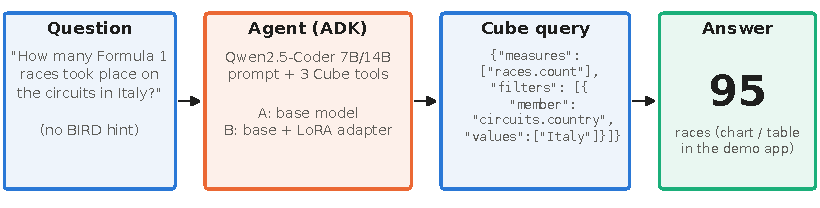
\includegraphics[width=0.7\linewidth]{figures/fig01_glance.pdf}
\caption{Project at a glance. A question goes to the agent, which writes a Cube query; Cube runs it and the rows become the answer (a stat tile here, a chart in the app). The two arms differ only in the LoRA adapter.}
\label{fig:glance}
\end{figure}

\section{Problem definition and proposed solution}

\subsection{Problem definition}
\begin{table}[!htbp]
\centering
\small
\caption{Definition of the task.}
\begin{tabularx}{0.95\linewidth}{@{}lX@{}}
\toprule
\textbf{Element} & \textbf{Definition}\\
\midrule
Intended user & An analyst or manager who asks questions in English about a known database.\\
Input & Question, BIRD hint (evidence) and the database name; the harness adds the Cube schema.\\
Required output & One Cube JSON query submitted with \texttt{submit\_answer}; its rows feed the chart.\\
Correct response & The query's rows equal the rows of BIRD's gold SQL on the original SQLite file (order of columns ignored).\\
Constraints & Local model on a 16\,GB GPU; at most 8 model calls per question; only names defined in the Cube models.\\
\bottomrule
\end{tabularx}
\end{table}

\subsection{Proposed solution}
The baseline is a \textbf{prompt-engineering harness}: a system prompt with a Cube query guide, rules and four worked examples, the database's Cube schema, and three tools (Fig.~\ref{fig:pipeline}). The harness also checks every query before it reaches Cube and replies with hints such as \emph{``did you mean races.count?''}. The proposed system adds a \textbf{LoRA adapter} trained on transcripts that use exactly this prompt and these tools, so the model learns the query language and the tool protocol from examples instead of reading them on every call. Fine-tuning suits the task because the output is strict JSON with exact names, and errors in the baseline were mostly format and protocol errors rather than missing knowledge.

\begin{figure}[!htbp]
\centering
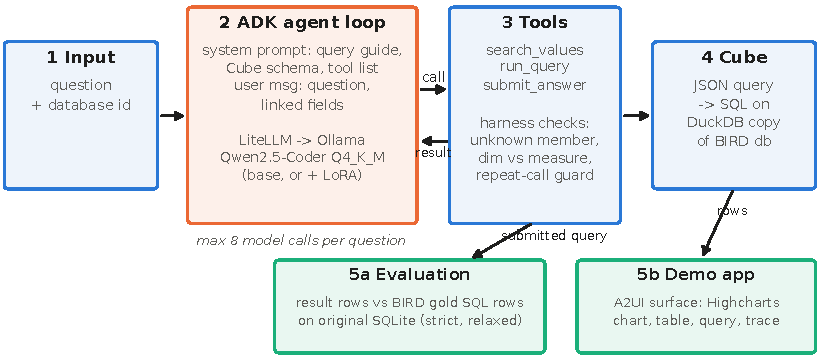
\includegraphics[width=0.76\linewidth]{figures/fig02_pipeline.pdf}
\caption{Steps from input to output. The agent loops between the model and the tools until it submits a query (max.\ 8 calls). The submitted query is scored against the gold SQL (5a) and shown as a chart in the demo app (5b). Every arm uses this same pipeline.}
\label{fig:pipeline}
\end{figure}

\subsection{Expected improvement}
The baseline's errors on development data were dimensions placed under \texttt{measures}, invented member names and malformed tool calls (Section~\ref{sec:method}). These are exactly what supervised examples teach well~\cite{patil2023gorilla}, so we expected (1) higher accuracy, (2) fewer steps per question and (3) that the query guide and tool definitions could be dropped from the prompt once the adapter has learned them~\cite{snell2022distilling}.

\section{Data}
\begin{table}[!htbp]
\centering
\small
\caption{Data used. All splits come from BIRD~\cite{li2023bird} (CC BY-SA 4.0). No database appears in more than one split.}
\begin{tabularx}{\linewidth}{@{}l>{\raggedright\arraybackslash}Xrr@{}}
\toprule
\textbf{Split} & \textbf{Purpose} & \textbf{Items} & \textbf{Databases}\\
\midrule
LoRA training & BIRD train questions turned into verified Cube transcripts & 3,273 & 55\\
LoRA validation & Same, three whole databases held out; early-stopping check only & 258 & 3\\
Harness tuning & BIRD dev questions used to develop the prompt and tools & 363 & 3\\
Final test & All BIRD dev questions on \texttt{formula\_1} (174) and \texttt{student\_club} (158); run once per arm & 332 & 2\\
\bottomrule
\end{tabularx}
\end{table}

\subsection{Source and preparation}
BIRD gives, for each question, an English question, an evidence hint, a gold SQL query and the SQLite database. We copied each database to DuckDB and generated a Cube model from its schema, foreign keys and BIRD's column descriptions. For training data, a rule-based translator turned each gold SQL query into a Cube query; we ran both and kept the pair only if the rows matched and were not empty (Fig.~\ref{fig:data}a). Each kept pair became a chat transcript with the harness's exact system prompt, the user message and the tool calls \texttt{run\_query} then \texttt{submit\_answer}; 769 transcripts also start with a \texttt{search\_values} call for a filtered text value. The loss is computed only on assistant turns.

\begin{figure}[!htbp]
\centering
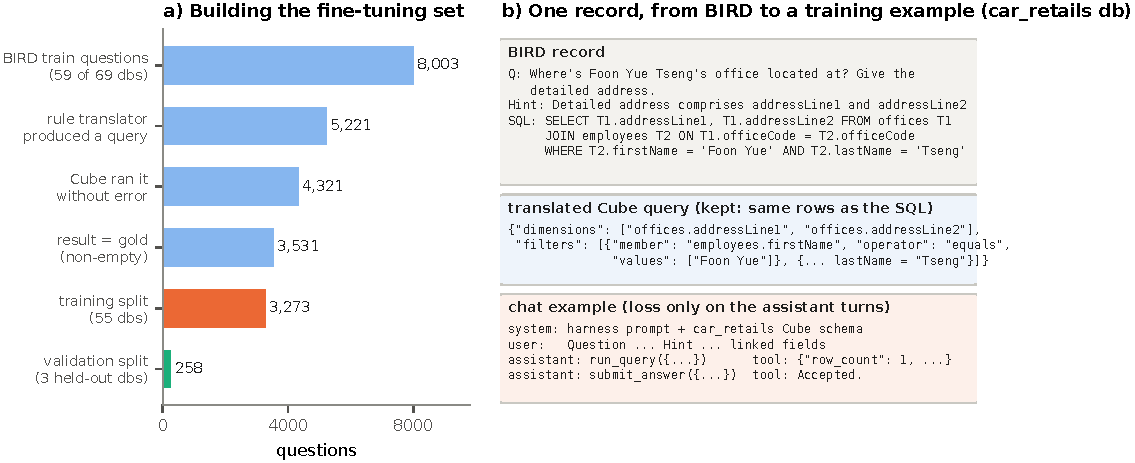
\includegraphics[width=0.78\linewidth]{figures/fig03_data.pdf}
\caption{(a) From 8,003 BIRD training questions to 3,531 verified examples: 2,782 used SQL a semantic layer cannot express, 900 failed in Cube and 790 gave different or empty results. (b) One record, its verified Cube query and the transcript the model is trained on.}
\label{fig:data}
\end{figure}

\subsection{Data quality and limitations}
The translator only handles SQL that Cube can express, so the training set has no subqueries, \texttt{CASE} arithmetic or string slicing; 30\% of the test questions need such SQL and are out of reach for any Cube query (the translator's own ceiling on the test set is 231/332). BIRD gold SQL has some errors and ties in \texttt{ORDER BY \dots LIMIT 1}. The test set is scored against the gold SQL's rows, not a reference Cube query, so any correct query counts. The ten largest training databases (over 600\,MB each) were skipped for disk and time.

\section{Method}\label{sec:method}

\subsection{Base model and baseline}
Both arms use \texttt{Qwen2.5-Coder-7B-Instruct} and \texttt{-14B-Instruct}~\cite{hui2024qwen25coder}, served by Ollama as Q4\_K\_M GGUF files with temperature 0 and a 16,384-token context. The baseline is the harness, improved over five versions on the tuning databases only (Fig.~\ref{fig:versions}). Version 2 added rules for the most common errors and four worked examples; v3--v4.2 added value lookup on number and date fields, \emph{schema linking} (the user message lists fields whose names match words in the question), a repeated-call guard and a column check before submission. Version 4.2 was frozen before any LoRA run.

\begin{figure}[!htbp]
\centering
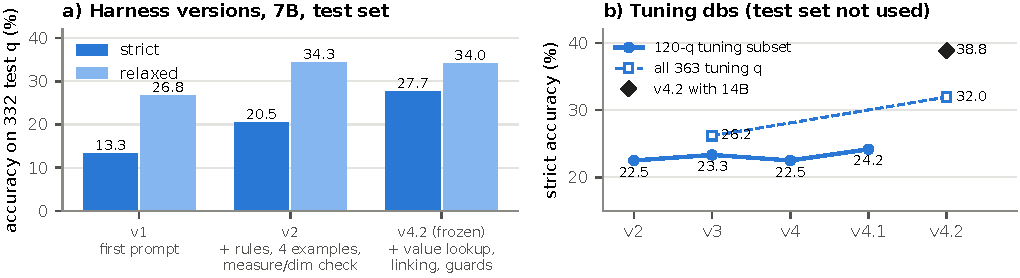
\includegraphics[width=0.8\linewidth]{figures/fig04_harness_versions.pdf}
\caption{Prompt-engineering progress for the 7B baseline. (a) The three versions that were also run on the test set: strict accuracy doubled from v1 to v4.2. (b) The development loop used only tuning databases; on all 363 tuning questions v4.2 beat v3 (32.0\% vs 26.2\%, McNemar $p{=}0.011$), and the 14B model reached 38.8\%.}
\label{fig:versions}
\end{figure}

\subsection{Chosen method}
We fine-tune with QLoRA~\cite{dettmers2023qlora} using PEFT~\cite{peft}: the base model is frozen in 4-bit NF4 and rank-16 adapters are added to all attention and MLP projections (Fig.~\ref{fig:method}). After training, the adapter is merged, converted to GGUF with llama.cpp~\cite{llamacpp} and quantised to the same Q4\_K\_M format as the base, with the base model's chat template, so the comparison isolates the adapter. To test how much of the prompt the weights can hold, we trained two more adapters per size on shorter prompts: \textbf{lean} drops the query guide, examples and tool JSON schemas and shortens the schema; \textbf{noschema} also drops the schema, which only works if the adapter has seen the test schemas, so its training set adds about 1,300 synthetic template questions on the two test databases (no BIRD dev question, hint or SQL is used).

\begin{figure}[!htbp]
\centering
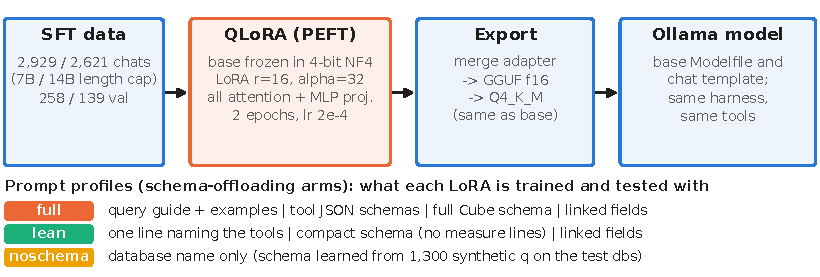
\includegraphics[width=0.75\linewidth]{figures/fig05_method.pdf}
\caption{Fine-tuning pipeline (top) and the three prompt profiles (bottom). Only the adapter and the prompt profile change between arms.}
\label{fig:method}
\end{figure}

\subsection{Implementation details}
\begin{table}[!htbp]
\centering
\small
\caption{Settings needed to reproduce the method.}
\begin{tabularx}{0.95\linewidth}{@{}lX@{}}
\toprule
\textbf{Setting} & \textbf{Value}\\
\midrule
Models & Qwen/Qwen2.5-Coder-7B-Instruct and -14B-Instruct (Hugging Face); Ollama \texttt{qwen2.5-coder:7b/14b} Q4\_K\_M\\
Agent & Google ADK 2.14 \texttt{LlmAgent} via LiteLLM~\cite{adk}; Cube on DuckDB; harness v4.2\\
LoRA & r=16, $\alpha$=32, dropout 0.05, q/k/v/o/gate/up/down projections, 4-bit NF4 base\\
Training & 2 epochs, lr $2\times10^{-4}$ cosine, warm-up 3\%, batch 1 $\times$ 16 accumulation, max.\ 8,192 tokens (7B) / 4,096 (14B, memory limit), seed 7\\
Generation & temperature 0, context 16,384 tokens, at most 8 model calls per question\\
Hardware & one RTX 5070 Ti (16\,GB), 32\,GB RAM, Windows; training 5.3\,h (7B) and 9.0\,h (14B)\\
\bottomrule
\end{tabularx}
\end{table}

\begin{figure}[!htbp]
\centering
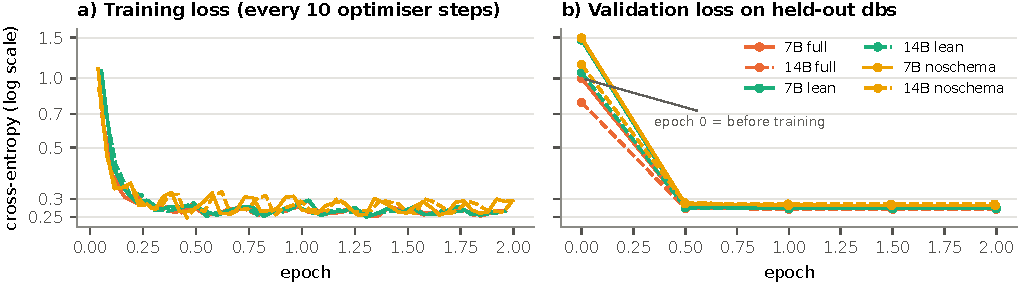
\includegraphics[width=0.78\linewidth]{figures/fig06_training.pdf}
\caption{Training progress for all six adapters. The loss drops within the first quarter epoch and then stays flat; validation loss on the three held-out databases follows it, so the adapters did not overfit. Lean and noschema adapters start higher because the model has never seen those short prompts.}
\label{fig:training}
\end{figure}

\section{Experiments}

\subsection{Compared systems}
\begin{enumerate}
  \item \textbf{Baseline:} base Qwen2.5-Coder 7B or 14B with harness v4.2 (full prompt, tools sent as JSON schemas).
  \item \textbf{Proposed system:} the same model file plus the LoRA adapter, same harness and prompt.
  \item \textbf{No-hint runs:} baseline and LoRA at both sizes again with BIRD's evidence hint hidden from the model (the adapters were trained with hints), closer to an analyst who types only a question.
  \item \textbf{Prompt-offloading arms:} LoRA trained and run with the \emph{lean} prompt; the \emph{noschema} LoRA run with no schema and with the lean prompt. As a control, the full-prompt LoRA was also given the lean prompt without retraining.
\end{enumerate}

\subsection{Evaluation data and measures}
The 332 test questions come from two databases unseen in training and tuning (218 simple, 91 moderate, 23 challenging; 77\% need a join).

\begin{table}[!htbp]
\centering
\small
\caption{Evaluation measures.}
\begin{tabularx}{\linewidth}{@{}l>{\raggedright\arraybackslash}X@{}}
\toprule
\textbf{Measure} & \textbf{How it is calculated}\\
\midrule
Strict accuracy (primary) & \% of the 332 questions whose rows and column count equal the gold SQL result\\
Relaxed accuracy & As strict, but extra columns are allowed (Cube must return any dimension it sorts by)\\
Prompt tokens / question & Prompt tokens summed over all model calls of one question\\
Steps, latency, speed & Model calls per question; model seconds per question (mean, median, 90th percentile); output tokens per model second\\
Tool use & Calls per tool, calls the harness or Cube turned back, and answers whose last draft returned no rows\\
Significance & Exact McNemar test on paired per-question outcomes (strict)\\
\bottomrule
\end{tabularx}
\end{table}

\subsection{Experimental procedure}
The test split and scoring rule were frozen first; the harness was developed on tuning databases only and frozen at v4.2. Each adapter was trained once (fixed seed) and each arm run once on all 332 questions. Within a size, all arms share the base model file, quantisation, context, temperature, step limit, tools and Cube models.

\section{Results}

\begin{table}[!htbp]
\centering
\footnotesize
\caption{Main results on the 332 held-out test questions. Tok./q: prompt tokens per question. $p$: McNemar, strict, against the harness-only arm of the same size.}
\label{tab:main}
\setlength{\tabcolsep}{4pt}
\begin{tabularx}{\linewidth}{@{}Xrrrrcrr@{}}
\toprule
\textbf{System} & \textbf{Strict\,\%} & \textbf{Relax.\,\%} & \textbf{Tok./q} & \textbf{Steps} & \textbf{Latency (s)} & \textbf{Tok./s} & $p$\\
 & & & & & {\scriptsize mean\,/\,med.\,/\,p90} & {\scriptsize output} & \\
\midrule
7B harness only (baseline) & 27.7 & 34.0 & 15,742 & 4.0 & 3.2\,/\,2.2\,/\,5.9 & 118 & --\\
7B LoRA + harness & \textbf{46.4} & \textbf{52.1} & 7,798 & 2.1 & 1.3\,/\,1.2\,/\,1.7 & 103 & $6{\times}10^{-11}$\\
7B lean LoRA & 41.9 & 45.5 & 3,257 & 2.2 & 1.3\,/\,1.2\,/\,1.6 & 109 & $1{\times}10^{-6}$\\
\midrule
14B harness only (baseline) & 28.9 & 41.3 & 10,766 & 2.9 & 4.0\,/\,3.5\,/\,5.7 & 67 & --\\
14B LoRA + harness & \textbf{49.7} & 56.9 & 7,341 & 2.0 & 2.5\,/\,2.4\,/\,3.3 & 58 & $3{\times}10^{-15}$\\
14B lean LoRA & 47.6 & \textbf{57.2} & 3,153 & 2.1 & 2.4\,/\,2.1\,/\,3.1 & 64 & $2{\times}10^{-12}$\\
\bottomrule
\end{tabularx}
\end{table}

\begin{figure}[!htbp]
\centering
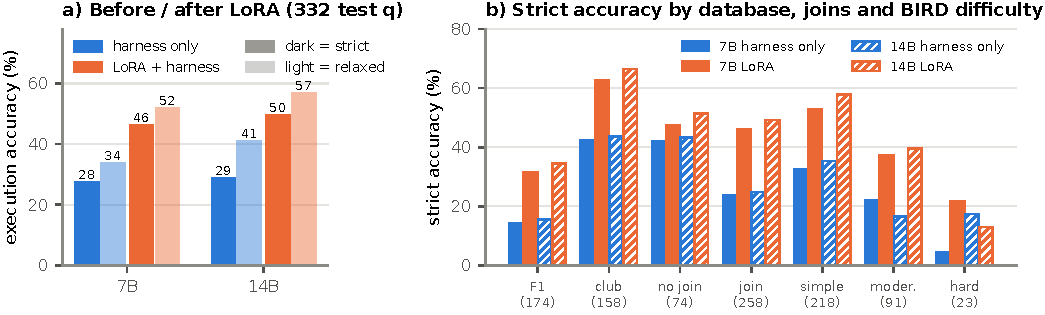
\includegraphics[width=0.68\linewidth]{figures/fig07_main.pdf}
\caption{Before and after fine-tuning (higher is better). (a) The LoRA adds about 20 points of strict accuracy at both sizes, more than doubling the model size does. (b) The gain holds on both databases and every difficulty level, and is largest on questions that need a join (7B: 24\% to 46\%).}
\label{fig:main}
\end{figure}

\subsection{Main findings}
The adapter is the main effect (Table~\ref{tab:main}, Fig.~\ref{fig:main}). At 7B it raised strict accuracy by 18.7 points: 78 questions became correct and 16 became wrong. At 14B the gain was 20.8 points (77 vs 8). The 7B LoRA beats the 14B baseline by 17.5 points, while the 14B LoRA is only 3.3 points above the 7B LoRA ($p{=}0.12$, not significant). The baseline 14B model has a much higher relaxed than strict score (41.3 vs 28.9): it often returns the right rows with extra columns, a habit the adapter mostly removed.


Fig.~\ref{fig:offload} answers the second part of the RQ. The lean LoRA sends 1.5k prompt tokens per call instead of 3.6--3.9k and loses 2.1 points at 14B ($p{=}0.21$, n.s.) but 4.5 points at 7B ($p{=}0.008$). Removing the schema entirely costs much more (14B: 38.3\%), because the model then invents members; adding the short schema back to the noschema adapter recovers 47.9\% (14B). A full-prompt LoRA given the lean prompt without retraining scored 0\%: the adapter learned its prompt, not the task in general.

\begin{figure}[!htbp]
\centering
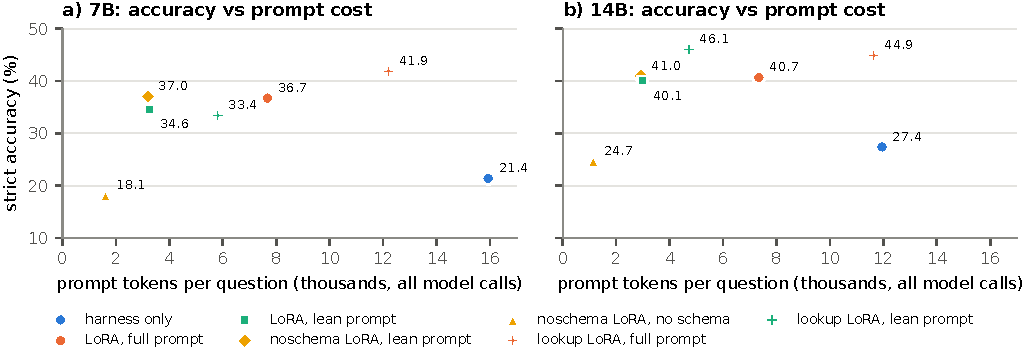
\includegraphics[width=0.74\linewidth]{figures/fig08_offload.pdf}
\caption{Accuracy against prompt cost (up and left is better). The lean adapters (green) keep most of the full LoRA's accuracy at 40\% of its prompt tokens; dropping the schema altogether (triangles) saves more tokens but loses 9--15 points.}
\label{fig:offload}
\end{figure}

\subsection{Without the hint}
\begin{table}[!htbp]
\centering
\footnotesize
\caption{Main arms with and without BIRD's hint, and tool use per question. $p$: McNemar (strict), without vs with hint. Lookups: \texttt{search\_values} calls; drafts: \texttt{run\_query} calls; rejected: calls the harness or Cube turned back; empty: answers whose last draft returned no rows.}
\label{tab:nohint}
\begin{tabularx}{\linewidth}{@{}Xlrrrrrrr@{}}
\toprule
\textbf{System} & \textbf{Hint} & \textbf{Strict \%} & \textbf{Relaxed \%} & $p$ & \textbf{Lookups} & \textbf{Drafts} & \textbf{Rejected} & \textbf{Empty \%}\\
\midrule
7B harness only & yes & 27.7 & 34.0 & -- & 1.59 & 0.86 & 0.83 & 3.0\\
 & no & 21.4 & 27.7 & 0.010 & 1.97 & 0.69 & 1.09 & 2.4\\
7B LoRA + harness & yes & 46.4 & 52.1 & -- & 0.00 & 1.09 & 0.13 & 7.5\\
 & no & 36.7 & 40.7 & $9{\times}10^{-7}$ & 0.01 & 1.09 & 0.11 & 13.0\\
\midrule
14B harness only & yes & 28.9 & 41.3 & -- & 0.66 & 0.94 & 0.10 & 10.5\\
 & no & 27.4 & 35.8 & 0.58 & 0.95 & 0.95 & 0.14 & 10.2\\
14B LoRA + harness & yes & 49.7 & 56.9 & -- & 0.00 & 0.98 & 0.00 & 5.4\\
 & no & 40.7 & 45.5 & $1{\times}10^{-6}$ & 0.00 & 0.97 & 0.00 & 13.3\\
\bottomrule
\end{tabularx}
\end{table}

Hiding the hint costs the adapters more than the baselines (Table~\ref{tab:nohint}): $-9.6$ and $-9.0$ points against $-6.3$ and $-1.5$ (n.s.). Trained with hints and never looking values up, the adapters guess more filter values and their empty answers double; the baselines look values up more often instead. The LoRA still leads by 15.3 (7B) and 13.3 points (14B), both $p{<}10^{-6}$. The 7B baseline spends its extra steps on rejected calls (0.8--1.1 per question vs about 0.1); the 14B models write most calls as text (71\%, 100\%), which the harness parses.

\subsection{Resource use}
Training took 5.3\,h (7B) and 9.0\,h (14B) on one 16\,GB GPU (lean: 2--3\,h) and converged within half an epoch (Fig.~\ref{fig:training}). The merged adapter adds no inference cost and halves the steps (4.0 to 2.1 at 7B), so prompt tokens halve and model time per question falls from 3.2 to 1.3\,s (p90: 5.9 to 1.7\,s). Output speed is unchanged (about 110 tokens/s at 7B, 60--65 at 14B), so the gain comes from fewer, shorter calls. Time to first token was not recorded, so prompt processing and decoding cannot be separated. Part of the saving comes from the adapter almost never calling \texttt{search\_values} (0.3\% of questions vs 92\%), which also causes errors (Section~\ref{sec:discussion}).

\section{Discussion}\label{sec:discussion}

\begin{figure}[!htbp]
\centering
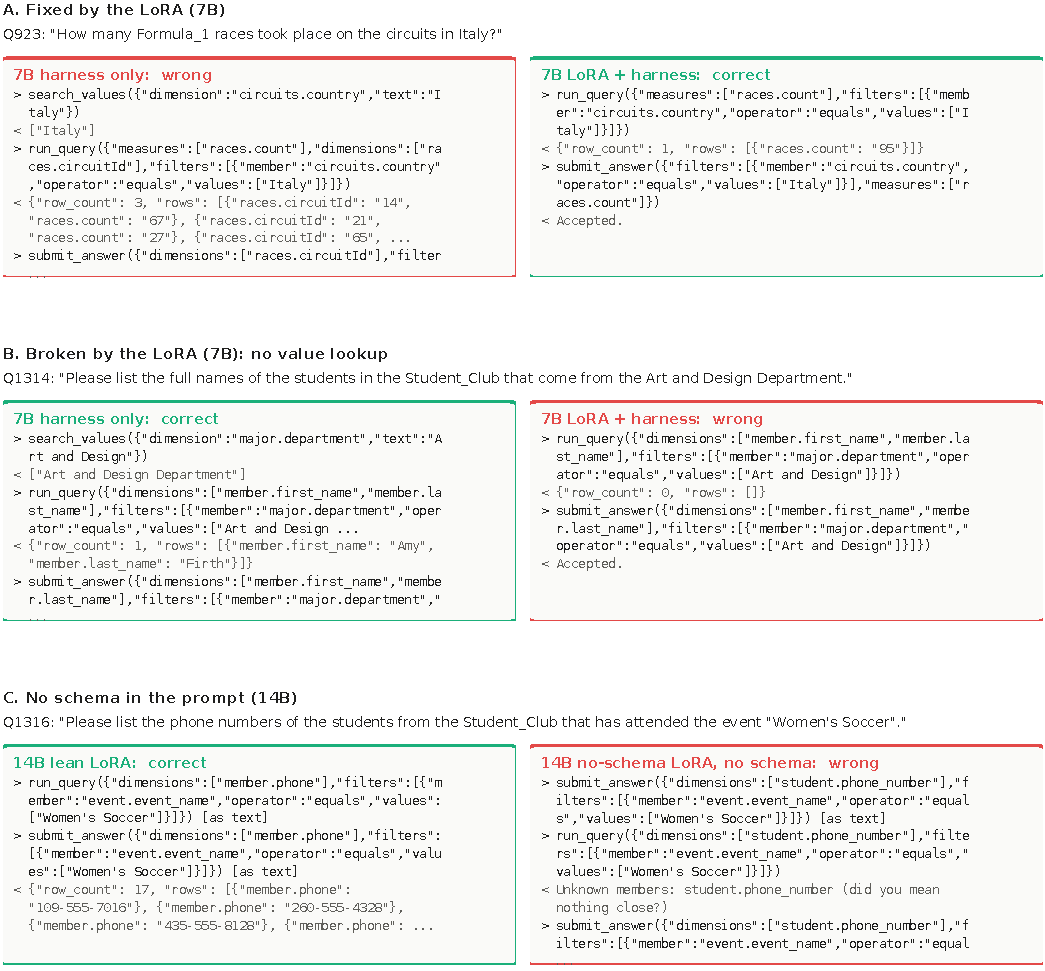
\includegraphics[width=0.7\linewidth]{figures/fig09_outputs.pdf}
\caption{Real tool traces from the test runs (\texttt{>} model call, \texttt{<} tool reply; long lines cut). A: the baseline groups by circuit and returns three rows, the LoRA asks for the single count. B: the LoRA skips the value lookup, filters on a value that does not exist and submits an empty result. C: without a schema the model invents \texttt{student.phone} and repeats it; the lean adapter writes \texttt{member.phone} (here as text, which the harness parses).}
\label{fig:outputs}
\end{figure}

\subsection{Interpretation and error analysis}
Fig.~\ref{fig:outputs} shows the typical change. The baseline follows its rules (it looks up ``Italy'' first) but then adds a grouping dimension that the question did not ask for, so the answer has three rows instead of one. Fig.~\ref{fig:errors} sorts every wrong answer into one category by fixed rules. The adapter almost removed failed runs (no valid query: 38 to 5 at 7B) and halved wrong filter values for the 14B model, while the share of questions that need SQL Cube cannot express stayed about 50: these are the ceiling of the approach, not a model error. The weak point is value lookup: only 22\% of training transcripts call \texttt{search\_values}, so the adapter learned to guess spellings (case B).

\begin{figure}[!htbp]
\centering
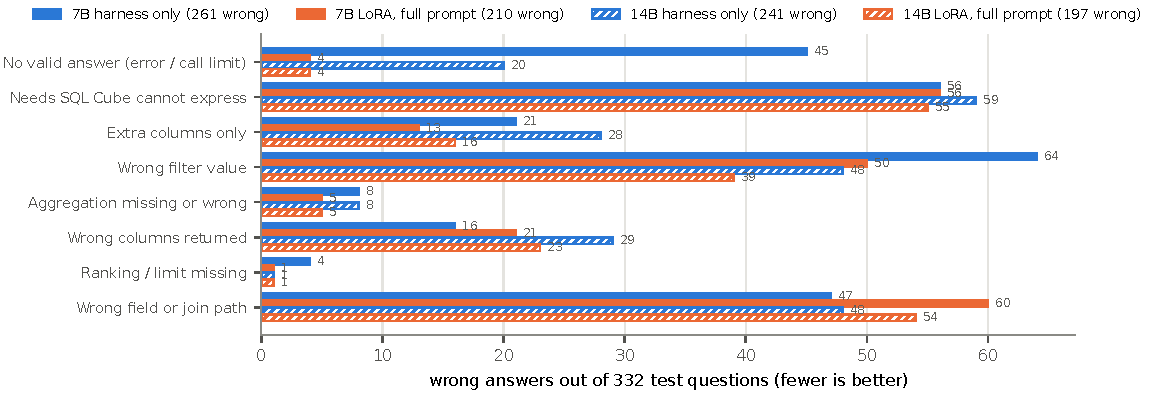
\includegraphics[width=0.62\linewidth]{figures/fig10_errors.pdf}
\caption{Wrong answers by category (rules applied in order). The LoRA mainly removes failed runs, wrong filters and extra columns; about 50 per arm need SQL Cube cannot express.}
\label{fig:errors}
\end{figure}

\subsection{Limitations and responsible use}
Two test databases and one run per arm give about $\pm$5 points of uncertainty (95\%). The translator limits training to queries Cube can express; the noschema arm is database-specific. The quantised 14B adapter writes a stray token instead of Qwen's \texttt{<tool\_call>} tag; the harness parses such text calls, but other clients would fail. BIRD is public and holds no private personal data. A chart from a wrong filter (case B) looks as convincing as a right one, so the demo app always shows the Cube query and tool trace beside it.

\section{Conclusion}
Keeping the harness fixed and adding a LoRA adapter trained on 3,273 execution-verified transcripts raised strict execution accuracy on unseen databases from 27.7\% to 46.4\% (7B) and from 28.9\% to 49.7\% (14B), halved the model calls per question, and made a 7B model beat a 14B one. Most of the prompt can move into the weights: a lean prompt kept the 14B model within 2 points at 40\% of the prompt tokens, but the schema must stay for unseen databases. Without BIRD's hint the adapters lose about 9 points but still lead by 13--15. The main limitation is that the adapter stopped looking up values. Next: retrain with \texttt{search\_values} in every transcript that filters on text and with some hints removed, and measure time to first token.

{\footnotesize
\let\oldthebibliography\thebibliography
\renewcommand\thebibliography[1]{\oldthebibliography{#1}\setlength{\itemsep}{0.1ex}}
\bibliographystyle{ce893}
\bibliography{references}
}
